%% Commands for TeXCount
%TC:macro \cite [option:text,text]
%TC:macro \citep [option:text,text]
%TC:macro \citet [option:text,text]
%TC:envir table 0 1
%TC:envir table* 0 1
%TC:envir tabular [ignore] word
%TC:envir displaymath 0 word
%TC:envir math 0 word
%TC:envir comment 0 0
%!TeX program = lualatex
\documentclass[acmsmall,authorversion]{acmart}
\usepackage{subcaption}
\usepackage{hyperref}
\usepackage[skins, breakable]{tcolorbox}
%% \BibTeX command to typeset BibTeX logo in the docs
\AtBeginDocument{%
  \providecommand\BibTeX{{%
    Bib\TeX}}}

\begin{document}

\title{Generative AI and Creativity: A Structure Literature Review and Meta Analysis}

\author{Niklas Holzner}
\email{n.holzner@campus.lmu.de}
\affiliation{
  \institution{LMU Munich}
  \city{Munich}
  \state{Bavaria}
  \country{Germany}
}
\author{Sebastian Maier}
\email{maier.sebastian@campus.lmu.de}
\affiliation{
  \institution{LMU Munich and Munich Center for Machine Learning (MCML)}
  \city{Munich}
  \state{Bavaria}
  \country{Germany}
}
\author{Stefan Feuerriegel}
\email{feuerriegel@lmu.de}
\affiliation{
  \institution{LMU Munich and Munich Center for Machine Learning (MCML)}
  \city{Munich}
  \state{Bavaria}
  \country{Germany}
}
\begin{abstract}
Generative artificial intelligence (GenAI) is increasingly used to support a wide range of human tasks, yet empirical evidence on its effect on creativity remains scattered. Can GenAI generate ideas that are creative? And to what extent can it support humans in generating ideas that are both creative and diverse? In this study, we conduct a meta-analysis to evaluate the effect of GenAI on the performance in creative tasks. For this, we first perform a systematic literature search, based on which we identify $N$ = XX relevant studies for inclusion in our meta-analysis. We then compute standardized effect sizes based on Cohen’s $d$. We compare different outcomes: (i)~how creative GenAI is; (ii)~how creative humans augmented by GenAI are; and (iii)~the diversity of ideas by humans augmented by AI. Our results indicate a small, statistically non-significant improvement in human creative performance ($d$ = X.XX), and a comparable but statistically significant creative performance for humans supported by GenAI ($d$ = X.XX). Further, GenAI has a positive effect on the diversity of ideas for such collaborations between humans and GenAI ($d$ = X.XX). We further analyze heterogeneity across different types of GenAI (e.g., ), different tasks (e.g., x), and participants (e.g., domain experts vs. laypeople). Overall, our results position GenAI as an augmentative tool that can support, rather than replace, human creativity---particularly in tasks benefiting from ideation support.
\end{abstract}

\maketitle
\section{Introduction}
\label{sec:Introduction}

\begin{itemize}
  \item \textbf{What GenAI can do:}  
    GenAI models learn statistical patterns from training data to synthesize novel, contextually coherent text, images, or audio outputs  \cite{FeuerriegelBISE2024}.  In a recent pre-registered Turing test, GPT-4.5 was identified as the human interlocutor 73 \% of the time—providing strong evidence that modern generative AI can closely approximate human conversational performance \cite{jones2025largelanguagemodelspass}.
    \item \textbf{AI in creative domains.}  
    Generative AI is already embedded in creative industries---spanning graphic design, advertising, fashion, writing, and visual arts---and supports multiple content modalities (text, image, video) through tools like ChatGPT, Midjourney, and Stability.AI \cite{Sun_2024}.
    \item \textbf{Research gaps (Opposite Hypothesis):} 
    There is various research that discusses effects of GenAI usage on the theoretical side. Most applied work surveys user attitudes or measures general productivity. However, can GenAI really excel at being creative? Transformer-based GenAI models show a steep drop in performance on tasks that require systematic, compositional reasoning such as multi‐step problem solving or hierarchical logic. They rely on surface pattern matching rather than true analytic structure \cite{Dziri2023FaithFate}. This suggests that, despite impressive generative fluency, GenAI may not consistently achieve the deeper conceptual integration that forms the basis of human creativity.
    \item \textbf{Early experimental findings:}  
        In controlled studies, using ChatGPT leads to more creative ideas than working without a tool or using a simple web search \cite{LeeChung2024}. Nevertheless there are only few works that test how GenAI changes originality or idea diversity across different tasks, people and domains as can be seen in our structured literature research. Here we thus compare the effect of GenAI across three different outcomes: difference between human and GenAI creative performance, effect of human-AI collaboration (HAIC) on creative performance and on creative diversity. 
    \item \textbf{By that we want to answer the following Research gaps:} \\
        \textbf{RQ 1:} How does GenAI alone compare to humans in creative performance in creativity tasks?
        \textbf{RQ 2:} How does using GenAI affect human creative performance in creativity tasks?\\
        \textbf{RQ 3:} How does using GenAI affect creative diversity in creativity tasks?\\
    \item \textbf{This paper’s contribution:}  
        To answer these questions we perform a systematic literature search and execute a meta-analysis on studies that directly compare human versus GenAI creative outputs or measure GenAI’s causal impact on human creative performance and creative diversity.
\end{itemize}
\begin{figure}[H]
  \centering
  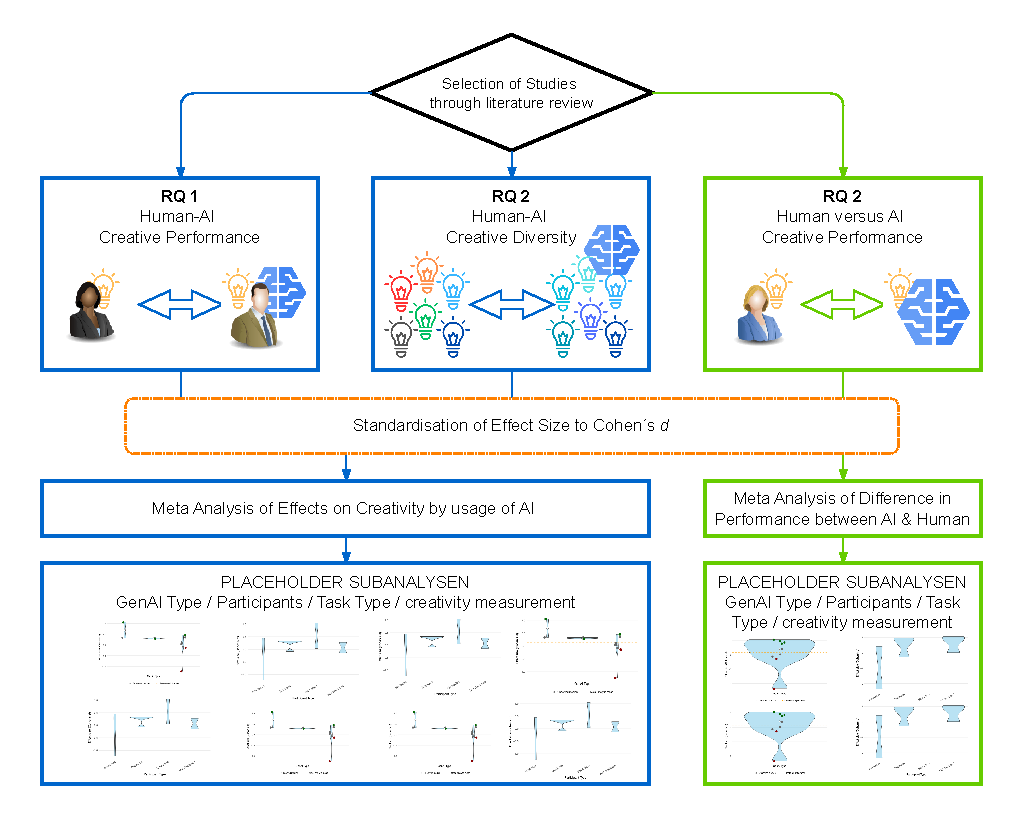
\includegraphics[width=\linewidth]{MetaAnalysis_LLM_Creativity_Research_Concept}
  \caption{Research concept visualized.}
  \Description{Research concept visualized.}
\end{figure}
\newpage
\section{Methods}
\label{sec:Methods}
\subsection{Data Collection}
\label{subsec:DataCollection}
\begin{itemize}
  \item \textbf{Meta-analytic framework.}  
    We follow the approach of Schemmer et al.\,(2022) to synthesize experimental evidence on human–GenAI co-creation \cite{Schemmer2022}.

  \item \textbf{Literature search.}  
    We conducted structured searches in Web of Science, SSRN and arXiv using combinations of  
\begin{figure}[ht]
  \centering
  \begin{tcolorbox}[
    enhanced,
    breakable,
    center upper, 
    colback=gray!10,
    colframe=gray!60!black,
    boxrule=0.8pt,
    arc=4pt,
    outer arc=4pt,
    drop shadow={black!50!white,opacity=0.3},
    width=\textwidth,
    title=\textbf{Database Search Query}
  ]
    \begin{verbatim}
("creativity" OR "creative" OR "ideation" OR "idea")
AND
("AI" OR "Artificial Intelligence" OR "LLM" OR "Large Language Models")
    \end{verbatim}
  \end{tcolorbox}
  \caption{Boolean search string used in literature databases.}
  \label{fig:search-query}
\end{figure}

    \item \textbf{Definitions:} Task types (AUT / DAT / ANOVA / etc.) 

\begin{table}[ht]
  \centering
  \label{tab:definitions}
  \begin{tabular}{l|p{7cm}|l}
    \toprule
    \textbf{Term} & \textbf{Definition} & \textbf{Source} \\
    \midrule
    Generative AI (GenAI) & AI systems that synthesize novel artifacts (text, images, audio) by learning patterns from data & \cite{FeuerriegelBISE2024}\\
    Human-AI collaboration (HAIC) &  & \\
    Creative performance & (Various Measures: novelty, originality, creativity) & \\
    Creative diversity &  & \\
    \addlinespace
    \bottomrule
  \end{tabular}
  \caption{Key definitions and sources.}
\end{table}

  \item \textbf{Inclusion criteria.}  
    We included studies that  
    \begin{enumerate}
      \item compared human creative performance with and without GenAI support, 
      \item compared human creative performance with AI creative performance, 
      \item reported sufficient statistics (means and standard deviations, error margins, or smiliar) for quantitative creativity measures,
      \item used a between-subjects experimental design.  
    \end{enumerate}

  \item \textbf{Study coding and data extraction.}  
    For each included paper, we extracted:  
    \begin{itemize}
      \item \emph{Participants}: sample size, domain 
      \item \emph{Creative domain}: writing, design, product ideation, etc.  
      \item \emph{GenAI type}: text-to-text (T2T), text-to-image (T2I)  ??? Mabey GPT-3 etc...
      \item \emph{Creativity measures}: fluency, originality, flexibility (e.g., AUT, DAT)  
    \end{itemize}

  \item \textbf{PRISMA documentation.}  
    We recorded the numbers of records identified, screened, included, and excluded following PRISMA guidelines; see Figure~\ref{fig:PRIMSAFlowchart} for the flowchart. Use of AI in the screening phase is declared in the flowchart.
\end{itemize}
\subsection{Statistical Analysis}
\label{subsec:DataCollection}
\begin{itemize}
  \item \textbf{Effect size calculation.}  
    We computed standardized mean differences (Cohen’s $d$) for each GenAI vs.\ control comparison, converting reported statistics as needed. For small samples ($n \le 20$), we applied Hedges’ $g$ correction to adjust for bias \cite{Hedges1985}.

  \item \textbf{Random‐effects meta‐analysis}  
    A random-effects model was estimated using the DerSimonian–Laird method to pool effect sizes and account for between-study variance ($\tau^2$) \cite{DerSimonian1986}. All analyses were implemented in R with the \texttt{metafor} package.

  \item \textbf{Heterogeneity assessment.(Thema mit Simon heute)}  
    We report the $I^2$ statistic and Cochran’s Q–test to quantify heterogeneity, and we present prediction intervals to indicate the expected range of true effects.

    (ist heterogeneity vs. moderator nicht da gleiche? Oder ist oben das eher einer robustness check gegen selection bias ??? )

  \item \textbf{Moderator analyses.}  
    We conducted subgroup meta-analyses to test whether effect sizes differ by  
    \begin{itemize}
      \item \emph{Creative task} (e.g., writing vs.\ design vs.\ art)
      \item \emph{Creative measurement} (e.g., fluency vs.\ originality vs.\ novelty)
      \item \emph{GenAI type} (T2T vs.\ T2I)  ??? Mabey GPT-3 etc...
      \item \emph{Participants} (e.g., education vs.\ science vs.\ business vs.\ creative )
    \end{itemize}
\end{itemize}

\begin{figure}[H]
  \centering
  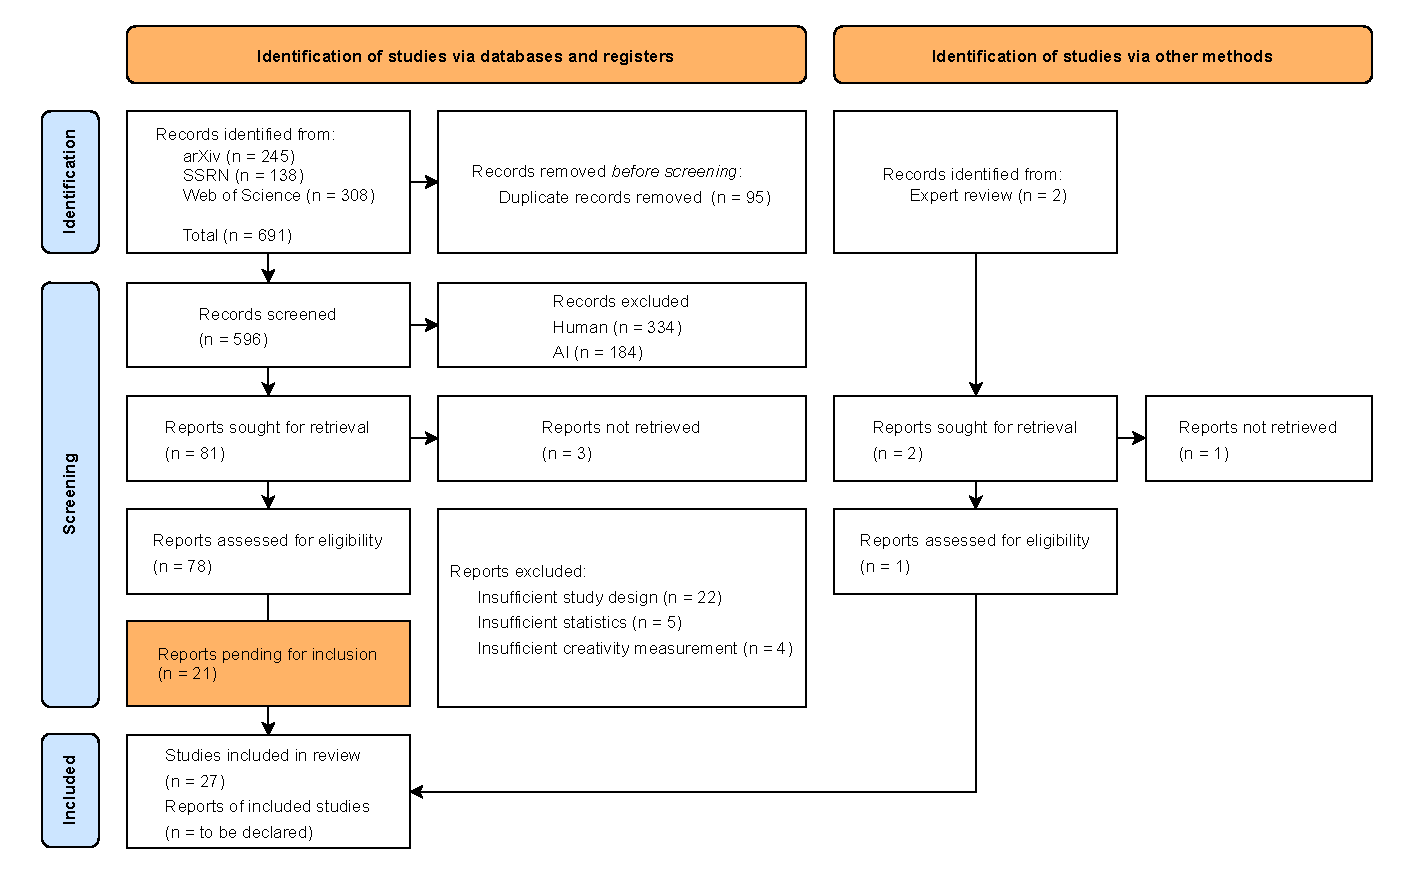
\includegraphics[width=\linewidth]{MetaAnalysis_LLM_Creativity_PRISMA_Flowchart.drawio}
  \caption{PRISMA Flow Chart}
  \Description{PRISMA Flow Chart of the Literature Research.}
  \label{fig:PRIMSAFlowchart}
\end{figure}

\begin{figure}[H]
  \centering
  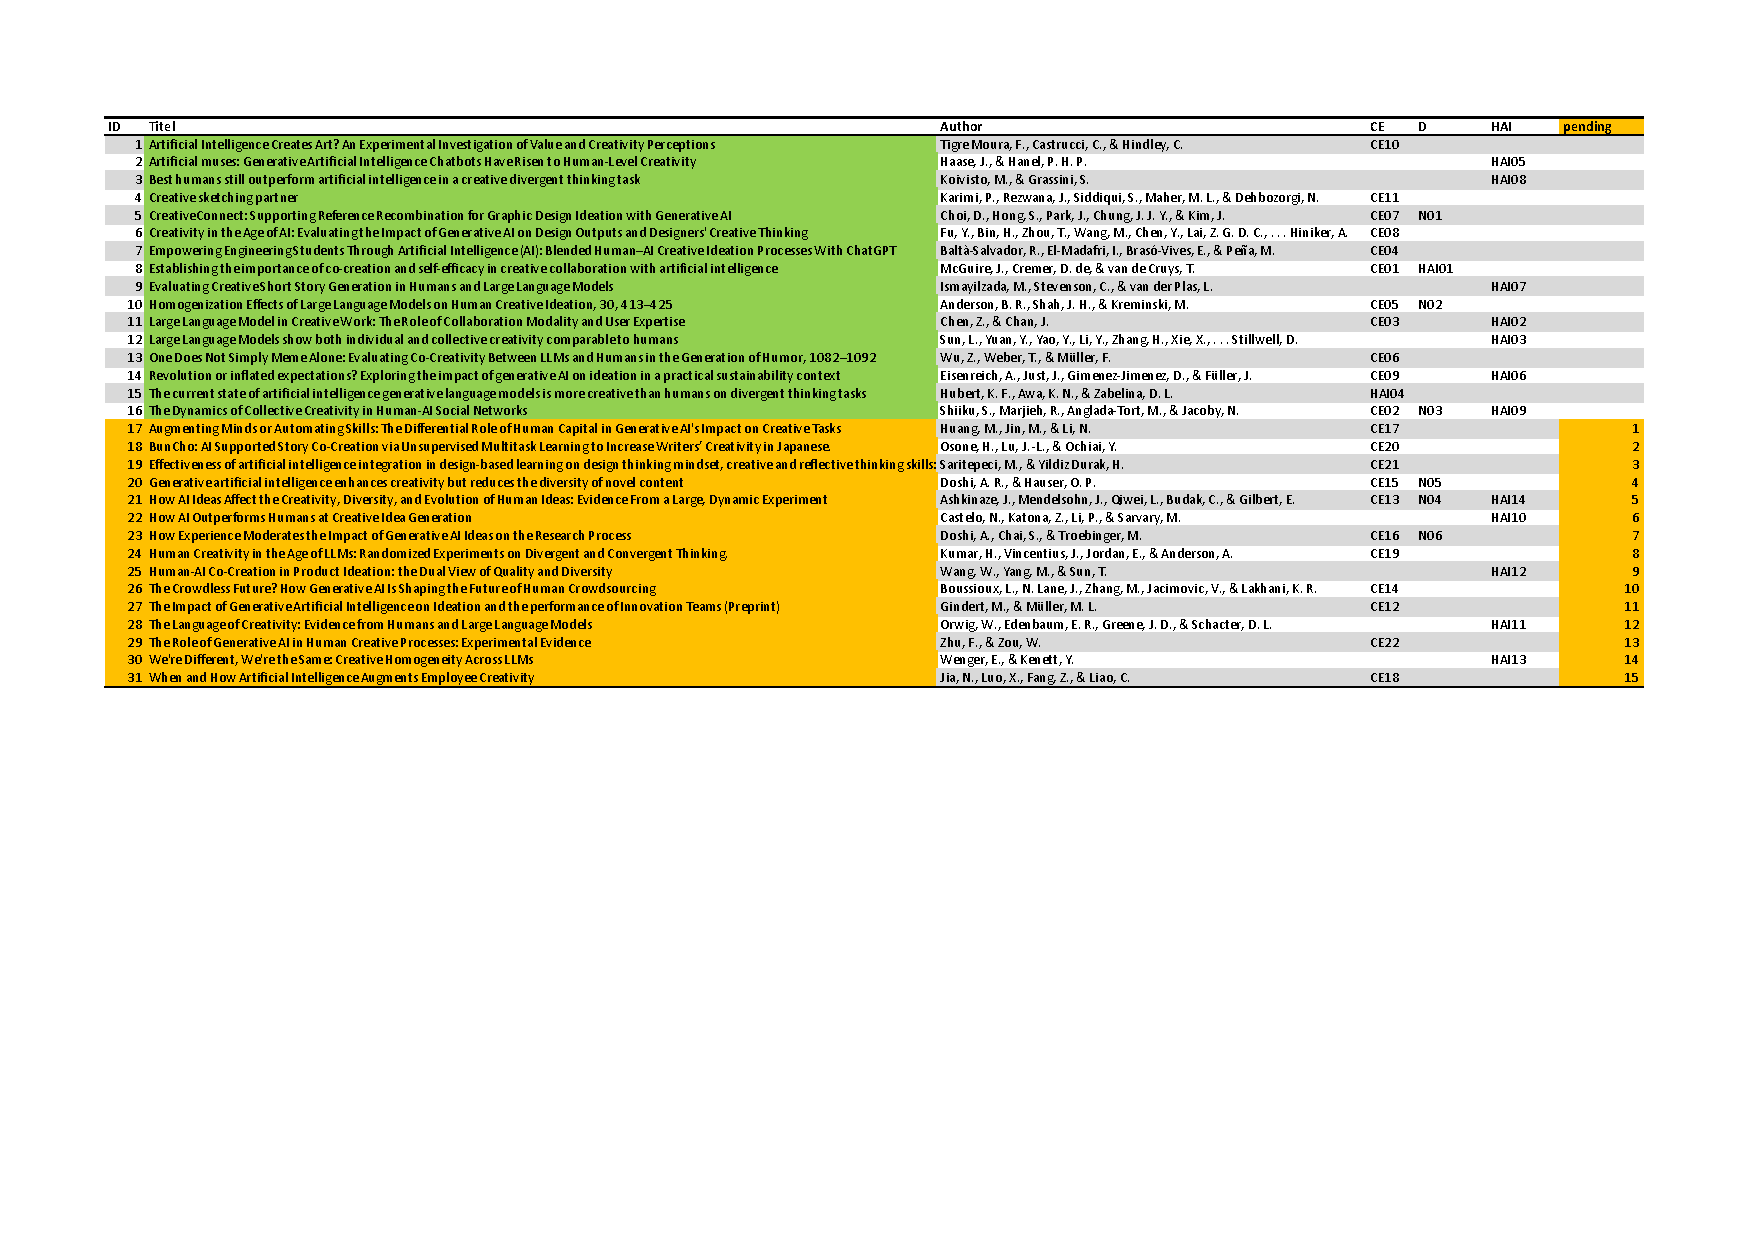
\includegraphics[width=\linewidth]{0_DRAFT List included Paper.pdf}
  \caption{List of Literature in Review.}
  \Description{List of Literature in Review.}
  \label{fig:TablePapers}
\end{figure}

\newpage


\section{Results}
\label{sec:Results}
\subsection{RQ 1 :Creative Performance Comparison of Human and AI}
\label{sec:CreativePerformanceComparisonOfHumanAndAI}
\textbf{RQ 1:} How does GenAI alone compare to humans in creative performance in creativity tasks? \\

\begin{itemize}
  \item \textbf{Forest Plot:} The overall effect size is small but positive (d = 0.149), with most individual studies non‐significant and a few showing significant positive or negative effects, reflecting modest heterogeneity in outcomes.
  \\ \\
  \item \textbf{Effect‐Size Distribution:} The violin plot shows a broad dispersion of effect sizes around the meta‐analytic mean, with substantial variability and some extreme negative values—yet the central tendency remains slightly positive, indicating that AI performance generally approximates human creativity.
  \\ \\
  \item \textbf{Moderator Analysis:} Participant background (business, education, undisclosed) does not significantly moderate the human–AI performance difference, as all subgroup confidence intervals overlap zero.
  \\ \\
  \item \textbf{Observed Funnel Plot:} The observed distribution of study effects is roughly symmetric around the pooled estimate, suggesting a low risk of publication bias.
  \\ \\
  \item \textbf{Trim‐and‐Fill Funnel Plot:} The trim‐and‐fill method imputes no additional studies, indicating minimal publication bias in the human–AI comparison literature.
  \\ \\
  \item \textbf{Overall Implication:} These analyses indicate that AI systems perform comparably to humans on creative tasks, with a small overall advantage but considerable variability—underscoring the value of AI as a complementary tool in creative workflows rather than a wholesale replacement.
\end{itemize}

\begin{figure}[H]
  \centering
  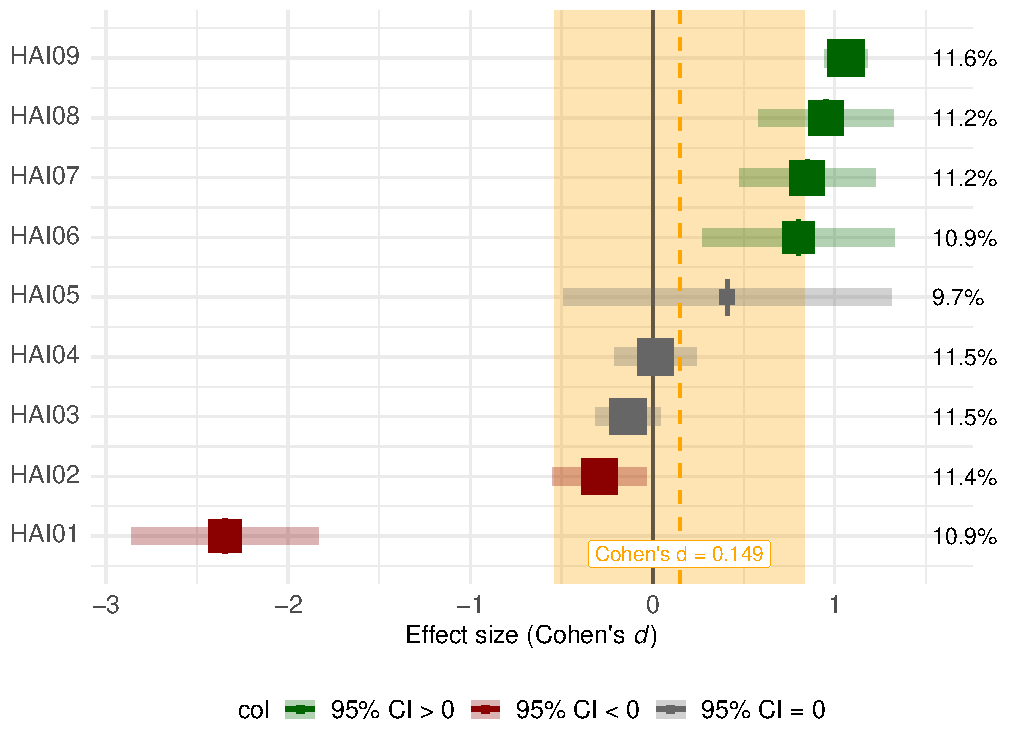
\includegraphics[width=\linewidth]{plot_versus_forest}
  \caption{Forest plot of human‐versus‐AI creative performance comparisons across 9 tasks (HAI01–HAI09), showing individual study Cohen’s $d$ and 95\% confidence intervals. The summary diamond at the bottom indicates an overall effect size of $d = 0.149$, suggesting a modest advantage for human outputs. The percentage next to each study name represents its relative weight in the meta‐analysis, and the vertical null line at $d=0$ helps quickly identify which studies favour humans (right side) or AI (left side).}
  \Description{Forest plot displaying individual Cohen’s d and 95\% confidence intervals for nine human‐AI comparison studies, plus overall summary effect of d = 0.149.}
  \label{fig:versus_forest}
\end{figure}

\begin{figure}[H]
  \centering
  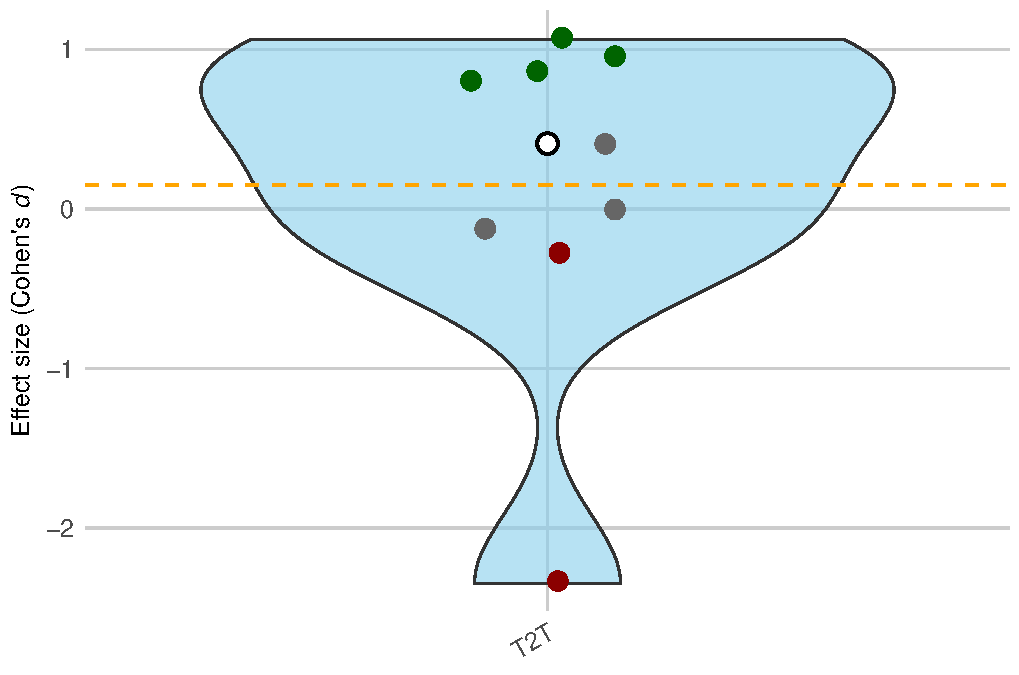
\includegraphics[width=\linewidth]{plot_versus_violin_GenAI}
  \caption{Violin plot of Cohen’s $d$ distributions for human‐versus‐AI performance, broken down by GenAI type (text‐to‐text only). The shape indicates the density of effect size estimates around each value, revealing how consistently text‐only AI systems compare to human creativity across studies.}
  \Description{Violin plot showing distribution of Cohen’s d for human-versus-AI performance by GenAI type: T2T.}
  \label{fig:versus_violin_GenAI}
\end{figure}

\begin{figure}[H]
  \centering
  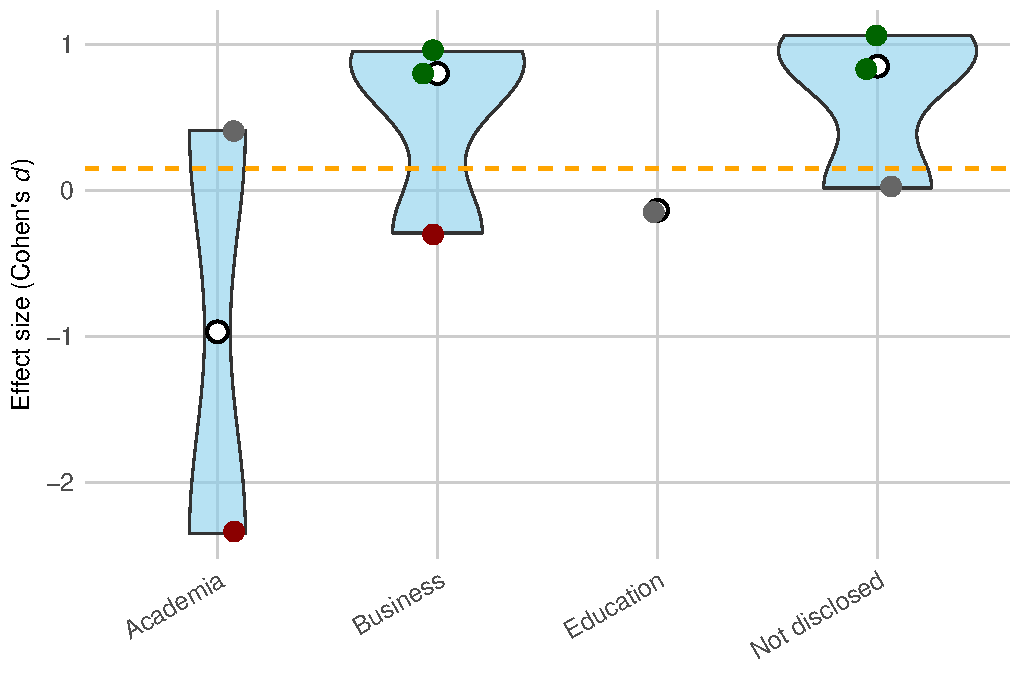
\includegraphics[width=\linewidth]{plot_versus_violin_participants}
  \caption{Violin plot showing the distribution of Cohen’s $d$ effect sizes for human‐versus‐AI performance across participant backgrounds (Academia, Business, Education, Not disclosed). The width at each $d$ value reflects how many estimates clustered there, providing insight into which populations show more pronounced or more variable differences in human versus AI outputs.}
  \Description{Violin plot displaying distribution of Cohen’s d for human-versus-AI performance across participant groups.}
  \label{fig:versus_violin_participants}
\end{figure}

\begin{figure}[H]
  \centering
  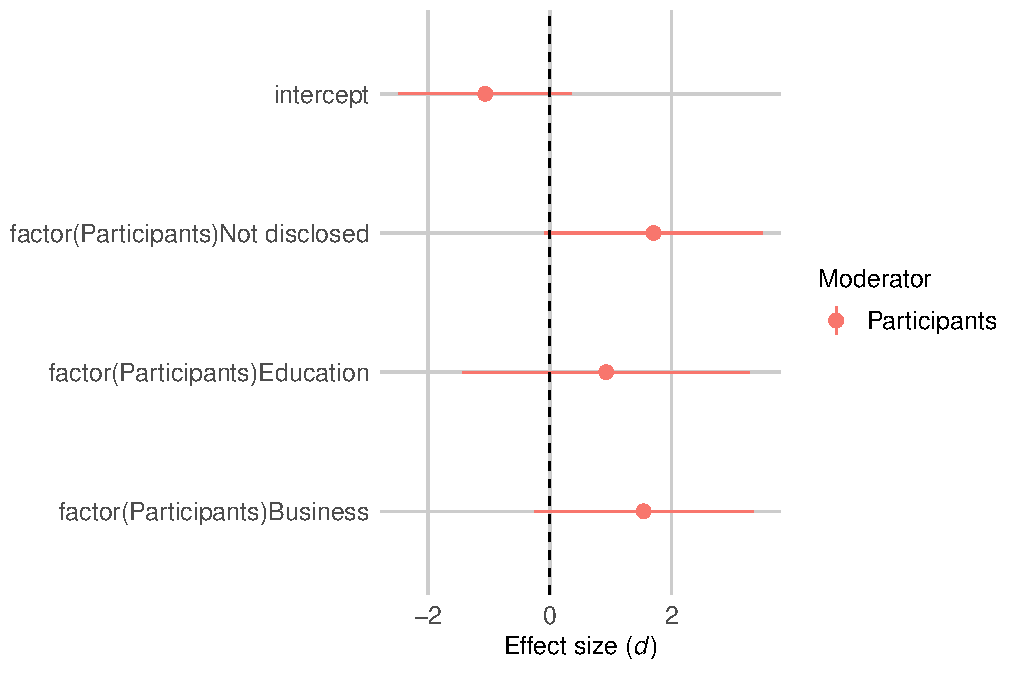
\includegraphics[width=\linewidth]{plot_versus_mod_plot}
  \caption{Moderator analysis for human‐versus‐AI performance showing Cohen’s $d$ estimates and 95\% confidence intervals across participant backgrounds (Business, Education, Not disclosed). The intercept represents the baseline text‐to‐text comparison effect, while subsequent rows show deviations for each group. This highlights how specific populations influence the magnitude of human versus AI performance differences.}
  \Description{Dot‐and‐whisker moderator plot displaying Cohen’s d and 95\% confidence intervals for participant group on human‐versus‐AI performance.}
  \label{fig:versus_mod}
\end{figure}
\newpage
\subsection{RQ 2 : Creative Performance}
\label{sec:CreativePerformance}
\textbf{RQ 2:} How does using GenAI affect human creative performance in creativity tasks? \\
\begin{itemize}
    \item \textbf{Forest Plot:} The overall effect size is small but positive (d = 0.128), with most individual studies non‐significant and a few showing significant positive or negative effects, reflecting modest heterogeneity in outcomes.
    \\ \\
    \item \textbf{Effect‐Size Distribution:} The violin plot shows a tight clustering of effect sizes around the meta‐analytic mean, with moderate variability and a slight skew toward positive effects—evidence of consistent, small enhancements in creative performance across studies.
    \\ \\
    \item \textbf{Moderator Analysis} Neither the type of generative AI (text‐to‐image vs.\ text‐to‐text) nor participant background (business, education, undisclosed) significantly alters the effect on creative performance, as all subgroup confidence intervals overlap zero.
    \\ \\
    \item \textbf{Observed Funnel Plot:} The observed distribution of study effects is reasonably symmetric around the meta‐analytic mean, further indicating low risk of publication bias.
    \\ \\
    \item \textbf{Trim‐and‐Fill Funnel Plot:} Imputed “missing” studies slightly adjust the pooled effect, suggesting only minimal publication bias in the literature on human–AI creative collaboration.
    \\ \\
    \item \textbf{Overall Implication:} Together, these analyses demonstrate that human–AI collaboration produces a reliably small enhancement in creative performance, with minimal bias and no major moderators—providing a solid empirical foundation for investigating how AI support can be optimally integrated to boost creativity in organizational settings.
\end{itemize}

\begin{figure}[H]
  \centering
  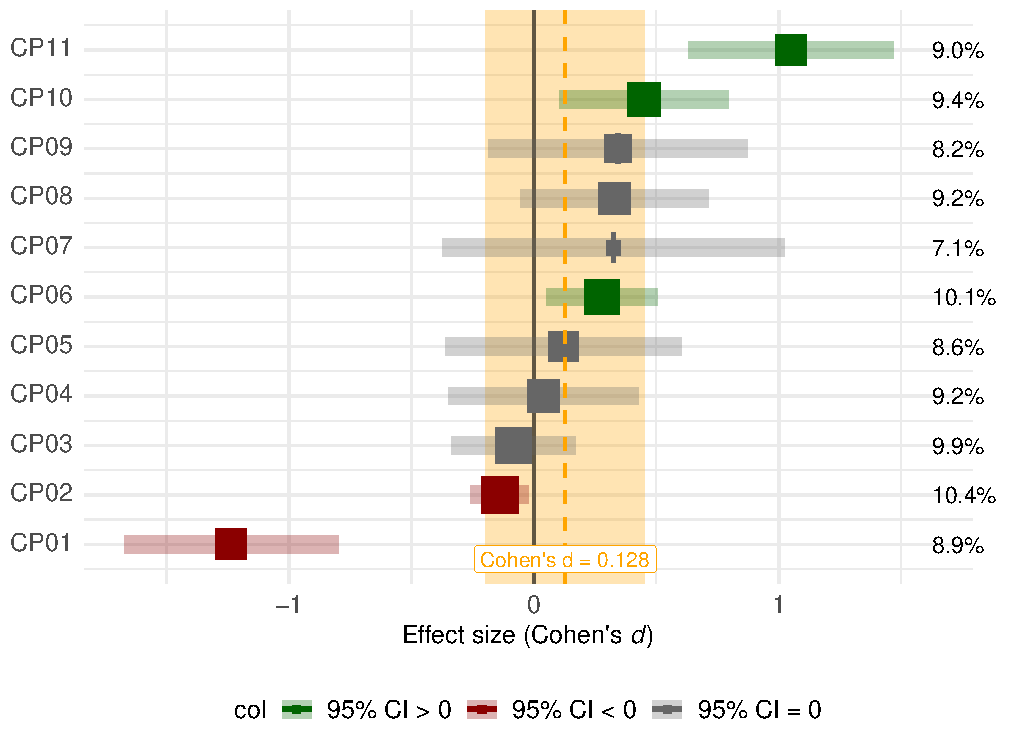
\includegraphics[width=\linewidth]{plot_performance_forest}
  \caption{Forest plot summarising the Cohen’s $d$ effect sizes and 95\% confidence intervals for human–AI creative performance across 11 distinct comparative tasks (CP01–CP11). Each horizontal line shows an individual study’s estimate (with its sample‐specific weight noted at the right), while the central diamond represents the overall summary effect size of $d = 0.128$, indicating a small but consistent advantage for human creative outputs over AI. The vertical line at $d=0$ marks the null effect, allowing quick visual comparison of which studies favour humans (right of the line) or AI (left of the line).}
  \Description{Forest plot displaying individual Cohen’s d and 95\% confidence intervals for human–AI creative performance (11 studies), plus overall summary effect of d = 0.128.}
  \label{fig:performance_forest}
\end{figure}

\begin{figure}[H]
  \centering
  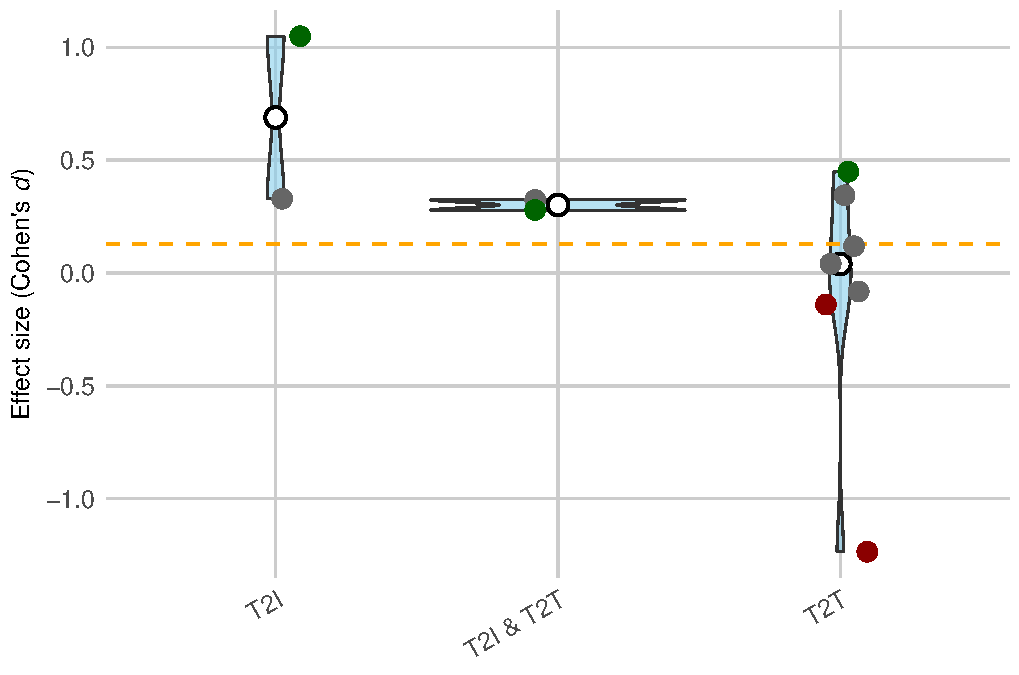
\includegraphics[width=\linewidth]{plot_performance_violin_GenAI}
  \caption{Violin plot depicting the full distribution of Cohen’s $d$ effect sizes for human–AI creative performance, stratified by GenAI system type: text‐to‐image (T2I), text‐to‐text (T2T), and hybrid (T2I + T2T). The width of each violin at a given $d$ value reflects the density of study estimates around that value, illustrating both central tendency and variability across system types. Median and interquartile spread can be inferred from the plot shape to compare consistency of effects between modalities.}
  \Description{Violin plot showing distribution of Cohen’s d for human–AI creative performance across three GenAI types: T2I, T2T, and T2I+T2T.}
  \label{fig:performance_violin_GenAI}
\end{figure}

\begin{figure}[H]
  \centering
  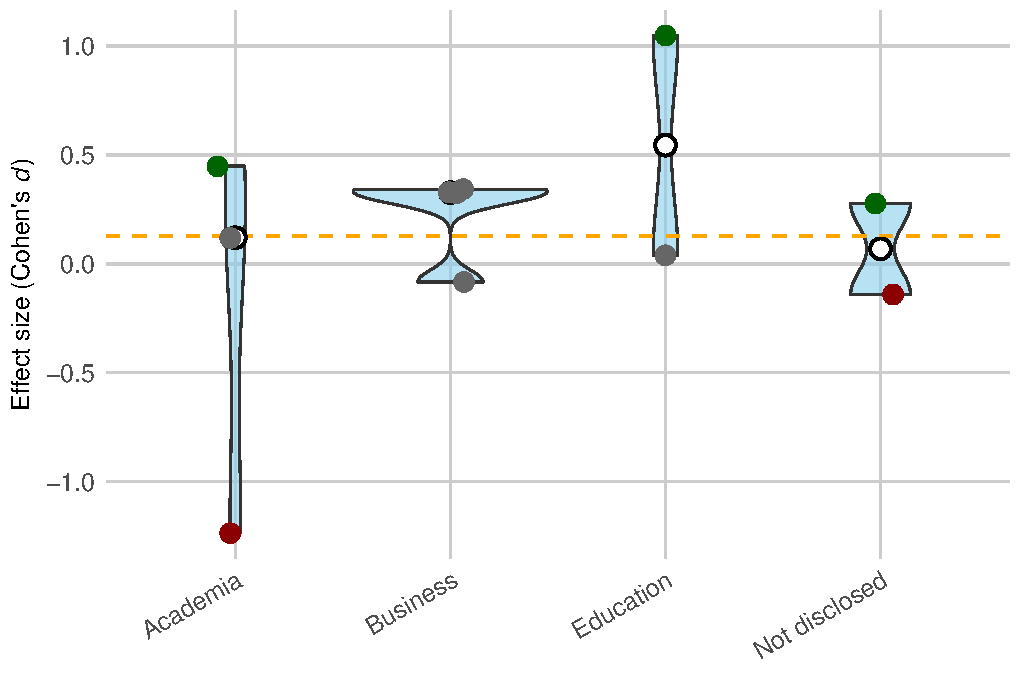
\includegraphics[width=\linewidth]{plot_performance_violin_participants}
  \caption{Violin plot illustrating the distribution of Cohen’s $d$ effect sizes for human–AI creative performance by participant background: Academia, Business, Education, and Not disclosed. Each violin’s shape reflects the density of observed effects, highlighting whether certain participant groups show more consistent or more variable performance differences when comparing human and AI creativity.}
  \Description{Violin plot showing distribution of Cohen’s d for human–AI creative performance across participant groups: Academia, Business, Education, Not disclosed.}
  \label{fig:performance_violin_participants}
\end{figure}

\begin{figure}[H]
  \centering
  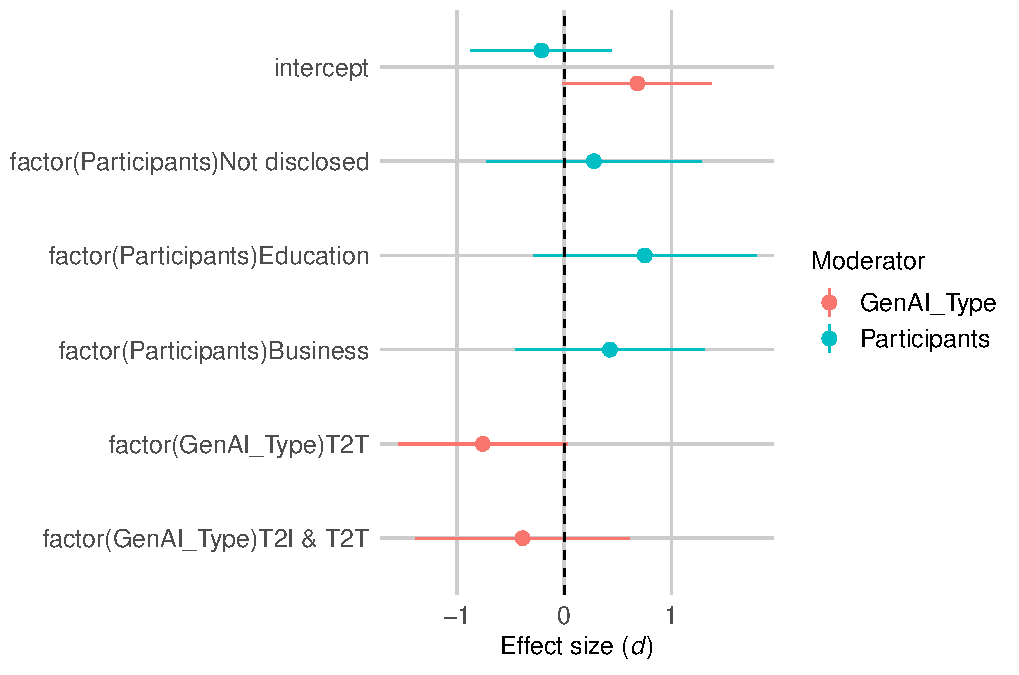
\includegraphics[width=\linewidth]{plot_performance_mod_plot}
  \caption{Moderator analysis of human–AI creative performance showing Cohen’s $d$ estimates for different levels of two categorical moderators: GenAI type (T2I + T2T vs.\ T2T alone) and participant background (Business, Education, Not disclosed). Points indicate estimated effect sizes, with horizontal bars denoting 95\% confidence intervals. The intercept at the top represents the baseline effect, while subsequent rows show how each subgroup deviates from that baseline, revealing which conditions amplify or attenuate the overall performance gap.}
  \Description{Dot‐and‐whisker moderator plot displaying Cohen’s d and 95\% confidence intervals for GenAI type and participant group on human–AI creative performance.}
  \label{fig:performance_mod}
\end{figure}
\newpage
\subsection{RQ 3 :Creative Diversity}
\label{sec:CreativeDiversity}

\textbf{RQ 3:} How does using GenAI affect idea diversity in creativity tasks? \\

\textbf{Strong limitation due to small amount of studies available}
\begin{itemize}
  \item \textbf{Forest Plot:} The overall effect size is large and positive (d = 0.638), with all included studies reporting either significant positive or non‐significant effects, indicating robust heterogeneity across outcomes.
  \\ \\
  \item \textbf{Moderator Analysis:} Subgroup analyses by AI type and participant background could not be conducted for creative diversity due to the limited number of studies, precluding formal tests of moderation.
  \\ \\
  \item \textbf{Observed Funnel Plot:} The observed funnel plot appears symmetric, suggesting low risk of publication bias among studies of AI’s effect on creative diversity.
  \\ \\
  \item \textbf{Trim‐and‐Fill Funnel Plot:} The trim‐and‐fill method imputes no additional studies, indicating minimal publication bias in the creative diversity literature.
  \\ \\
  \item \textbf{Overall Implication:} These analyses indicate that AI significantly enhances creative diversity with large effect sizes and minimal bias, highlighting strong potential for AI tools to diversify ideation processes in practice.
\end{itemize}

\begin{figure}[H]
  \centering
  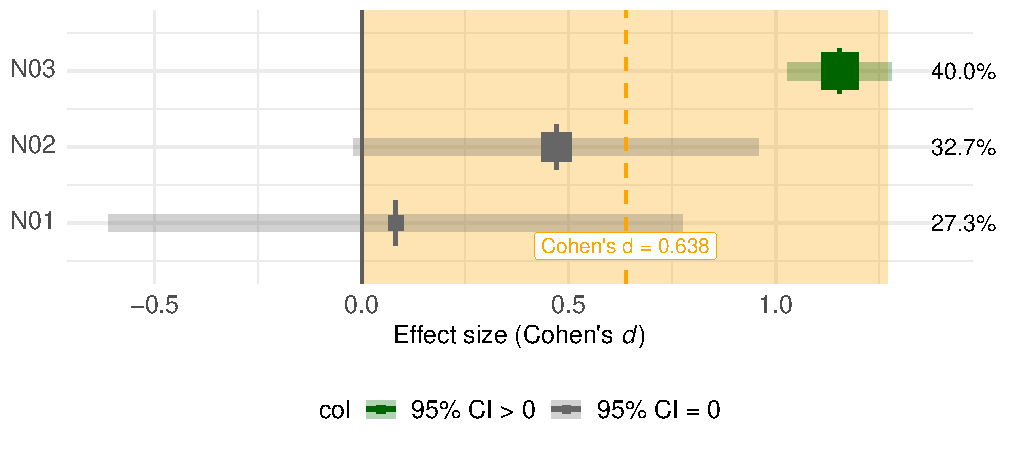
\includegraphics[width=\linewidth]{plot_diversity_forest}
  \caption{Forest plot of diversity metrics comparing human and AI outputs across three studies (N01–N03), with individual Cohen’s $d$ and 95\% confidence intervals. The overall summary effect of $d = 0.638$ indicates that AI‐generated content exhibits substantially higher diversity compared to human‐produced material. The vertical zero line helps visualise which studies show greater diversity in AI (right side) or human (left side) outputs.}
  \Description{Forest plot displaying individual Cohen’s d and 95\% confidence intervals for diversity comparisons (three studies), plus overall summary effect of d = 0.638.}
  \label{fig:diversity_forest}
\end{figure}

\newpage


\subsection{Overall Results}
\label{sec:CreativePerformanceComparisonOfHumanAndAI}
\begin{itemize}
    \item \textbf{Human versus AI (RQ 1):} The comparison shows a small, non‐significant AI advantage (d = 0.149, 95\% CI [–0.539, 0.836], p = 0.672) across 9 studies, with significant heterogeneity (Q(8) = 10.00, p < 0.001, I\textsuperscript{2} = 98.4\%, tau \textsuperscript{2} = 1.058) 
  \\ \\
  \item \textbf{Creative Performance (RQ 2):} The meta‐analysis yields a small, non‐significant effect (d = 0.128, 95\% CI [–0.196, 0.452], p = 0.439) across 11 studies, but with high heterogeneity (Q(10) = 78.45, p < 0.001, I\textsuperscript{2} = 91.5\%, tau \textsuperscript{2} = 0.258)
  \\ \\
  \item \textbf{Creative Diversity (RQ 3):} A large, significant effect emerges (d = 0.638, 95\% CI [0.005, 1.270], p = 0.048) across 3 studies, accompanied by substantial heterogeneity (Q(2) = 316.54, p < 0.001, I\textsuperscript{2} = 85.2\%, tau \textsuperscript{2} = 0.257)
  \\ \\
  
  \item \textbf{Overall Implication:} These findings suggest that AI tools are best conceived as performance amplifiers rather than substitutes for human creativity. The modest but consistent AI‐augmented gains in performance underscore that context, task design, and the specific capabilities of AI systems critically determine the magnitude of benefit—highlighting the need to tailor AI integrations to settings where human–AI synergies can maximize creative outcomes. 
\end{itemize}

\begin{figure}[H]
  \centering
  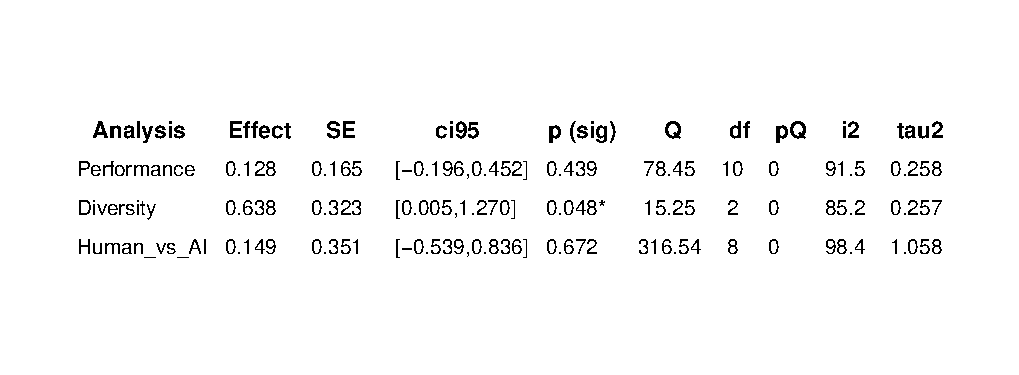
\includegraphics[width=\linewidth]{table_all_meta_analyses_results}
  \caption{Summary table of all meta‐analytic results.}
  \Description{Table summarizing k (number of studies), pooled effect size, standard error, 95\% CI, p‐value (with significance), Q statistic, degrees of freedom, I\^2, and tau\^2 for the three analyses: Performance, Diversity, and Human\_vs\_AI.}
\end{figure}
\newpage
\section{Discussion}
\label{sec:Discussion}

\begin{itemize}
    \item \textbf{Recap Relevance Marketing / Entertainment / Business} Embedding AI into operating models and workflows can amplify human performance by automating routine tasks and enabling human–AI symbiosis, thereby unlocking efficiency and innovation in core processes \citep{DavenportRonanki2018}.  
    \\ \emph{Suggested reference:} Artificial Intelligence for the Real World; Davenport \& Ronanki, 2018 (https://hbr.org/2018/01/artificial-intelligence-for-the-real-world?utm\_source=chatgpt.com)
\\ \\
    \item \textbf{Discussion Findings}    \\
    \textbf{RQ 1:} How does GenAI alone compare to humans in creative performance in creativity tasks? \\ Why is the GenAI creative performance close to humans performance?\\
    \textbf{RQ 2:} How does using GenAI affect human creative performance in creativity tasks? \\ Why is creative performance impact small?\\
    \textbf{RQ 3:} How does using GenAI affect idea diversity in creativity tasks? \\ Why is creative diversity probably not rising from LLM usage (mention limitation of this study again)?\\
    \\
    \item \textbf{Implications} What are the implications we can derive from our results for GenAI usage of humans and GenAI implementation in business (Focus on Strategy / Marketing \& Entertainment) 
\\ \\
    \item \textbf{Future Research} How to improve Human-AI collaboration and how you amplify GenAI creativity
\end{itemize}
\textbf{Human–AI teamwork:}  
    \begin{itemize}
         \item \textbf{Lubart (2005)} AI tools can act as creative partners. Lubart (2005) describes four computer roles—nanny, pen-pal, coach, colleague—with the “colleague” role sharing idea generation with humans \cite{LUBART2005365}.  
         \item \textbf{Dellermann et al. (2019)} show how hybrid-intelligence systems combine human judgment and AI predictions to improve innovation decisions \cite{Dellermann2019}.
    \end{itemize}
\begin{itemize}
        \item No direct quotes (!). No HBR (because there is no 'evidence' (you can use the ref in your discusison)\begin{quote}
          “Large language and image AI models have created a new set of opportunities for businesses and professionals that perform content creation” (Davenport \& Mittal, 2022). \url{https://hbr.org/2022/11/how-generative-ai-is-changing-creative-work}
        \end{quote}
        \item Industry reports show studios and media companies using AI to draft storylines, develop character arcs and even prototype basic scripts from a few prompts.  
        \begin{quote}
          “AI tools can suggest storylines, character arcs, and dialogue; [they] even include an interactive module that lets readers see for themselves how easily ChatGPT can write a basic script when given a few prompts” (MIT Sloan Management Review, 2023).  \url{https://sloanreview.mit.edu/article/the-impact-of-generative-ai-on-hollywood-and-entertainment/} 
        \end{quote}
        \item \begin{quote}
          “Generative AI significantly boosts artists’ productivity and leads to more favorable evaluations from their peers, increasing peak content novelty while reducing average novelty” (PNAS Nexus, 2024).  \url{https://academic.oup.com/pnasnexus/article/3/3/pgae052/7618478}
        \end{quote}
    \end{itemize}
\section{Conclusion}
\label{sec:Conclusion}

\begin{itemize}
  \item \textbf{Overall Conclusion:} AI‐augmented creativity yields small but consistent performance gains and, in particular contexts, substantial diversity boosts. However, these benefits materialize only when AI capabilities, task design, and organizational support are carefully aligned—underscoring that AI functions as an enhancer of human creativity rather than a replacement for it.
\end{itemize}
\newpage
\bibliographystyle{ACM-Reference-Format}
\bibliography{metaanalysis_llm_creativity}
\newpage
\appendix
\section{Terminology}

\begin{table}[ht]
\centering
\caption{Glossary of Key Terms}
    \label{tab:Terminology}
    \begin{tabular}{c p{5cm} l l}
        \toprule
        \textbf{Term} & \textbf{Definition} & \textbf{Abbreviation} & \textbf{Source}\\
        \midrule
        Generative AI & AI systems that produce novel content (text, images) from prompts & GenAI & Common\\
        Human-AI Collaboration &  Human‑AI Collaboration is the cooperative partnership between individuals and AI systems in order to accomplish common goals. & HAIC & \cite{fragiadakis2025evaluatinghumanaicollaborationreview} \\
        Creative Performance & - & - & - \\
        Creative Diversity & - & - & - \\
        \bottomrule
    \end{tabular}
\end{table}

\section{Additional statistical Analysis}
\subsection{Creative Performance Comparison of Human and AI}

\begin{figure}[H]
  \centering
  \begin{subfigure}[b]{0.49\linewidth}
    \centering
    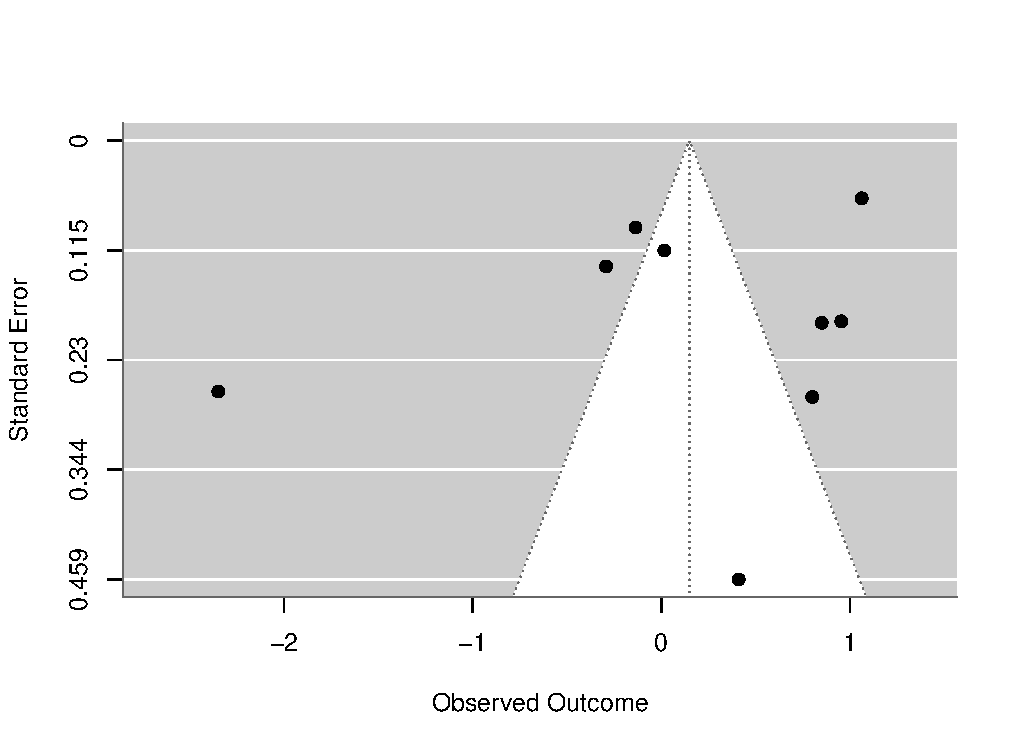
\includegraphics[width=\linewidth]{plot_versus_funnel_observed}
    \caption{Observed funnel plot for human–versus–AI performance}
  \end{subfigure}%
  \begin{subfigure}[b]{0.49\linewidth}
    \centering
    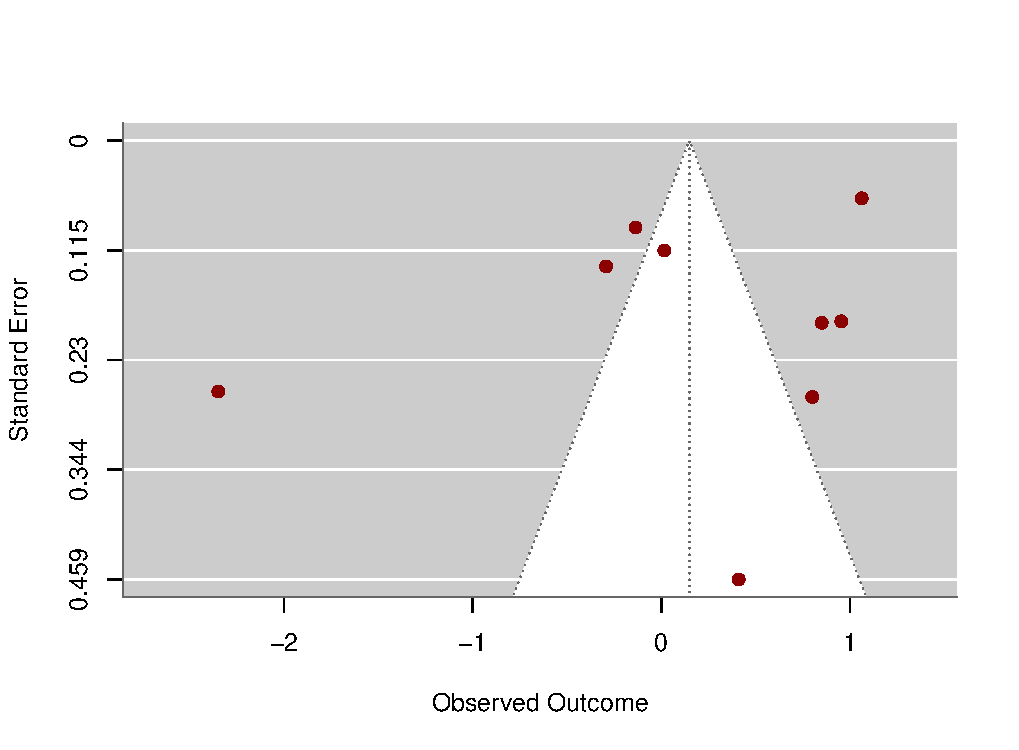
\includegraphics[width=\linewidth]{plot_versus_funnel_trimfill}
    \caption{Trim-and-fill funnel plot with imputed comparison studies in red}
  \end{subfigure}
  \caption{Funnel plots of human–versus–AI creative performance (9 studies). In (a), each study’s Cohen’s $d$ is plotted versus its standard error to form the classic funnel shape; deviation from symmetry suggests bias. In (b), the trim-and-fill method adds red‐colored “missing” studies to re‐centre the funnel and adjust the overall effect estimate, illustrating how small or unpublished comparisons could influence conclusions.}
  \Description{Left: observed funnel plot showing Cohen’s d versus standard error for human–AI comparisons; right: corresponding trim-and-fill funnel plot with imputed studies in red.}
  \label{fig:versus_funnels}
\end{figure}

\subsection{Creative Performance}
\begin{figure}[H]
  \centering
  \begin{subfigure}[b]{0.49\linewidth}
    \centering
    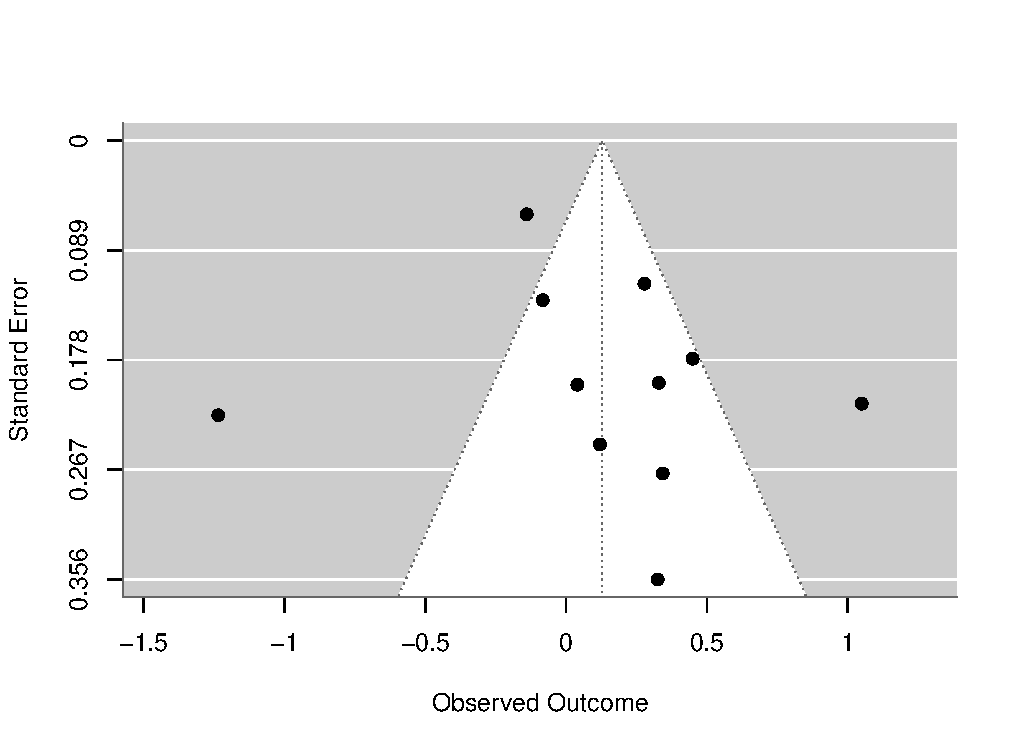
\includegraphics[width=\linewidth]{plot_performance_funnel_observed}
    \caption{Observed funnel plot for human–AI creative performance}
  \end{subfigure}%
  \begin{subfigure}[b]{0.49\linewidth}
    \centering
    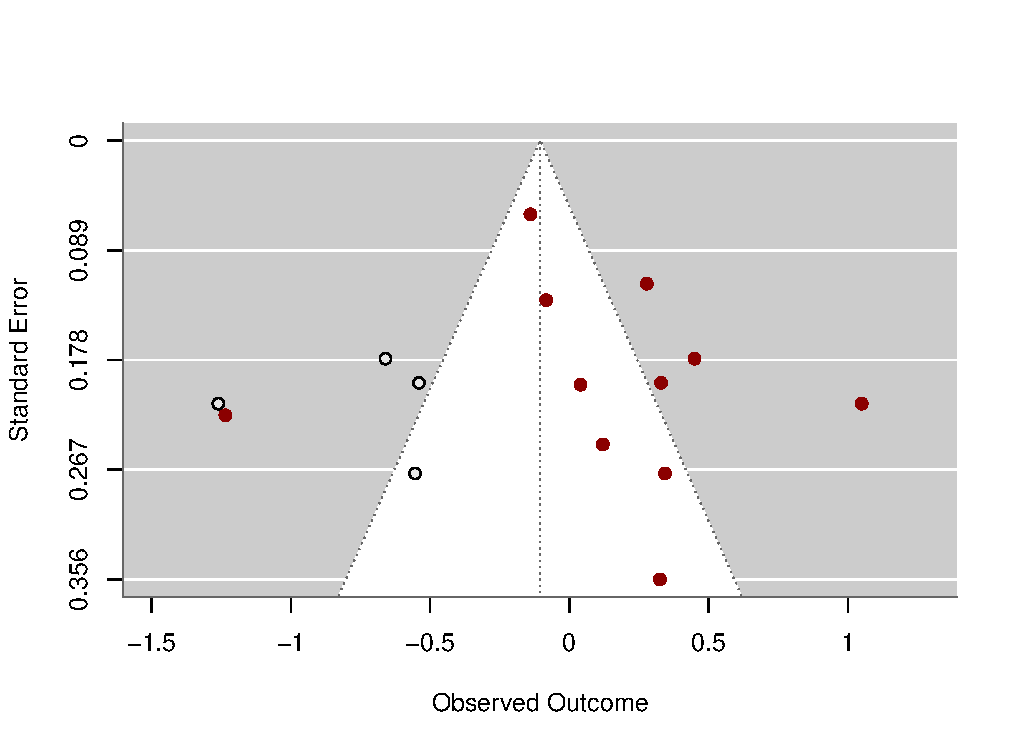
\includegraphics[width=\linewidth]{plot_performance_funnel_trimfill}
    \caption{Trim-and-fill funnel plot with imputed studies shown in red}
  \end{subfigure}
  \caption{Funnel plots of human–AI creative performance (11 studies). In (a), each point represents a study’s Cohen’s $d$ plotted against its standard error, with the funnel shape (dashed lines) delineating the 95\% confidence boundaries under no bias. In (b), the trim-and-fill algorithm imputes missing studies (in red) to achieve symmetry, adjusting the summary effect and highlighting potential publication bias toward larger effects.}
  \Description{Left: observed funnel plot showing each study’s standard error against its Cohen’s d; right: trim-and-fill funnel plot with imputed studies in red.}
  \label{fig:performance_funnels}
\end{figure}


\subsection{Creative Diversity}
\begin{figure}[H]
  \centering
  \begin{subfigure}[b]{0.49\linewidth}
    \centering
    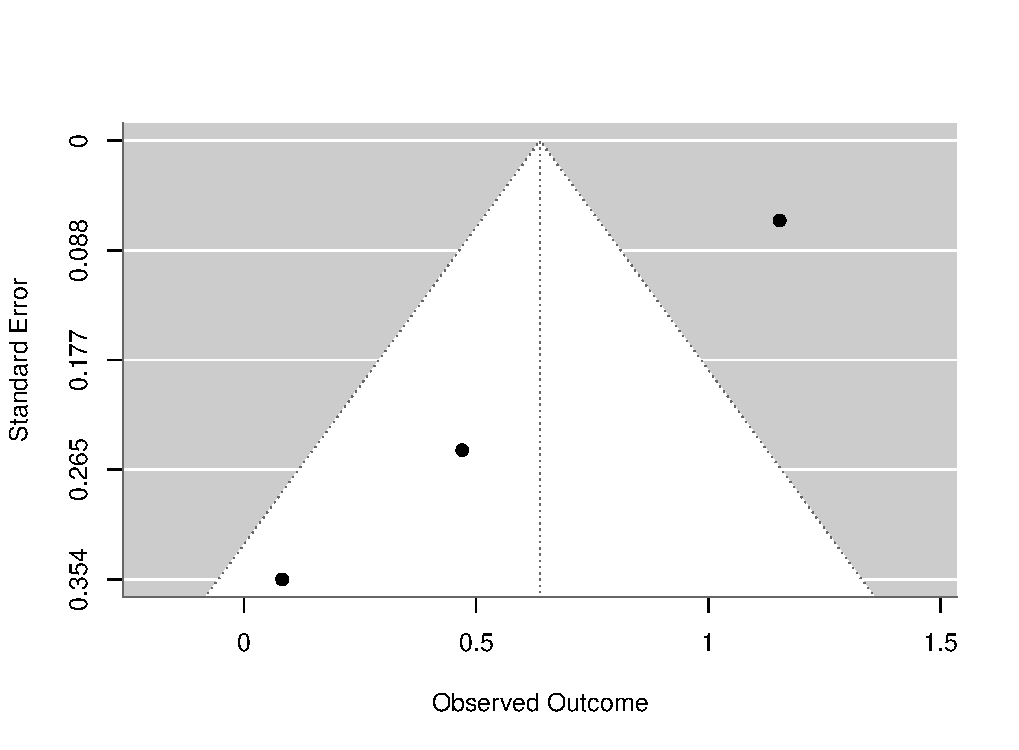
\includegraphics[width=\linewidth]{plot_diversity_funnel_observed}
    \caption{Observed funnel plot for diversity comparisons}
  \end{subfigure}%
  \begin{subfigure}[b]{0.49\linewidth}
    \centering
    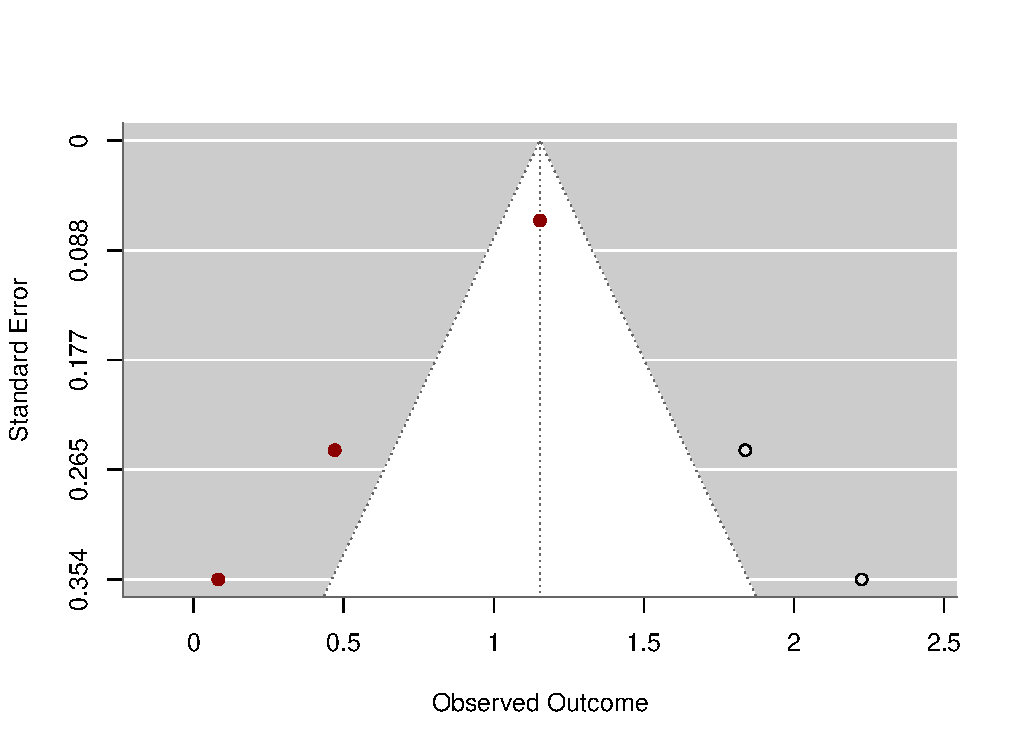
\includegraphics[width=\linewidth]{plot_diversity_funnel_trimfill}
    \caption{Trim-and-fill funnel plot with imputed diversity studies in red}
  \end{subfigure}
  \caption{Funnel plots of diversity metrics comparing human and AI outputs (3 studies). Panel (a) shows each study’s Cohen’s $d$ against its standard error, with the expected funnel contours indicating no bias. Panel (b) presents the trim-and-fill result: red points are imputed to correct asymmetry, yielding a more balanced estimate and revealing whether smaller or nonsignificant studies may be missing.}
  \Description{Left: observed funnel plot of diversity Cohen’s d vs standard error; right: trim-and-fill funnel plot with imputed diversity studies in red.}
  \label{fig:diversity_funnels}
\end{figure}

\end{document}